\chapter{Normalisation}
\label{ch:normalisation}

\section{Required reading}\label{required-reading}

\begin{enumerate}
\item
  Wikipedia article on
  \href{https://en.wikipedia.org/wiki/Database_normalization}{database
  normalisation}.
\item
  Textbook \citep{connolly:2015:database} Chapter 14 (Normalisation).
\item
  Original paper by Codd.
\end{enumerate}

\section{Normalisation}\label{normalisation}

\citet{connolly:2015:database} defines normalisation as:

\begin{quote}
A technique for producing a set of relations with desirable properties,
giving the data requirements f an enterprise.
\end{quote}

\subsection{Desireable properties}

\begin{itemize}
\item
  Minimise the number of attributes
\item
  Attributes with close logical relationship (functionally dependent)
  should be in same relation (table)
\item
  Minimal redundancy: data represented once, except for enabling joins
  on primary keys / foreign keys.
\end{itemize}

\subsection{Benefits}

\begin{itemize}
\item
  Minimdal redundancy means updates affect fewer attributes and
  relations meaning reduced number of operations.
\item
  Reduction in disk storage.
\item
  Avoidance of anomalies
\end{itemize}

\newpage
\section{Anomalies}\label{anomalies}

Redundant data causes anomalies where data manipulation operations are
not applied to all instances of the data.

\subsection{Update}\label{update}

An update anomaly arises where an update does not modify all instances
of specific data, .

\begin{figure}[htbp]
\centering
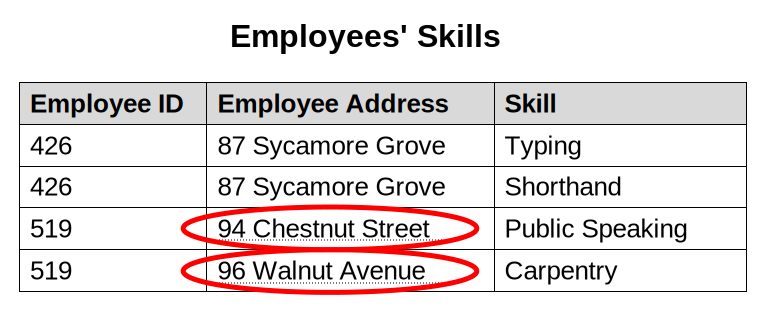
\includegraphics[width=0.5\linewidth]{update_anomaly}
\caption{Update anomaly (Wikipedia){}}
\end{figure}

\subsection{Insertion}\label{insertion}

An insertion anomaly arises where an insert causes either nulls to be
required to create a dummy record, .
An insert that causes inconsistency with existing data also is
identified as an insertion anomaly.

\begin{figure}[htbp]
\centering
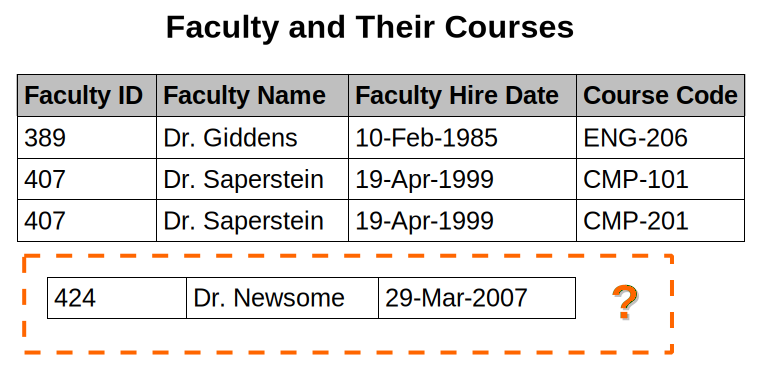
\includegraphics[width=0.5\linewidth]{insertion_anomaly}
\caption{Insertion anomaly (Wikipedia){}}
\end{figure}


\subsection{Deletion}\label{deletion}

A deletion anomaly arises where data is lost about one entity when
another entity is deleted, .

\begin{figure}[htbp]
\centering
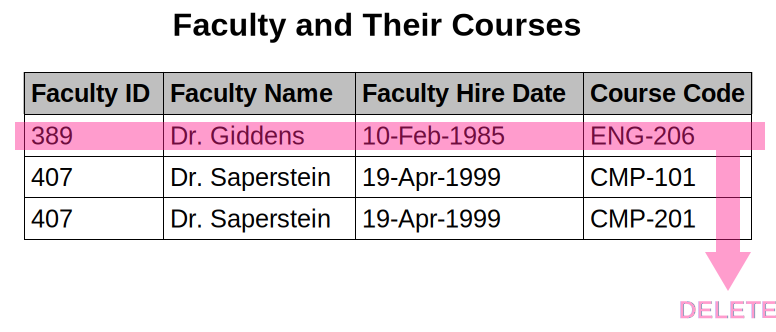
\includegraphics[width=0.5\linewidth]{deletion_anomaly}
\caption{Deletion anomaly (Wikipedia){}}
\end{figure}

\newpage

\section{Functional dependency}\label{functional-dependency}

If \(A\) and \(B\) are attributes of a relation \(R\), \(B\)
functionally depends on \(A\) if every value of \(A\) is associated with
one value of \(B\).

\begin{itemize}
\item
  Can say \(A\) functionally determines \(B\).
\item
  Would say \(A\) is the determinant in the relationship
\end{itemize}

\subsection{Full / partial functional
dependency}\label{full-partial-functional-dependency}

Let \(A\) and \(B\) be attributes of a relation \(R\):

\begin{description}
\item[Full functional dependency]
is where \(B\) functionally depends on \(A\), but not any proper subset
of \(A\).
\item[Partial functional dependency]
exists where \(B\) functionally depends on \(A\) and on one or more
proper subsets of \(A\).
\end{description}

\subsection{Characteristics}\label{characteristics}

When normalising, functional dependencies should:

\begin{enumerate}
\def\labelenumi{\arabic{enumi}.}
\item
  Have 1:1 relationship between determinant and the functional
  dependent.
\item
  Hold for all time.
\item
  Be full (not partial), i.e.~have minimum number of attributes
  necessary
\end{enumerate}

\subsection{Transitive dependency}\label{transitive-dependency}

Let \(A, B, C\) be attributes of a relation \(R\). Assume that \(A\)
isn't functionally dependent on \(B\) or \(C\).

If \(A \Rightarrow B\) and \(B \Rightarrow C\) then \(C\) is
transitively dependent on \(A\).

\section{Primary key}\label{primary-key}

A primary key must be UNIQUE and NOT NULL.

\subsection{Simple}\label{simple}

Simple primary key is one that involves only ONE column.

Any column directly defined as a \texttt{PRIMARY\ KEY} will be a simple
primary key.

\subsection{Compound}\label{compound}

A compound key is a primary key composed of more than 1 column.

\subsection{Candidate keys}\label{candidate-keys}

In practice there may be a number of possible columns and groups thereof
that could be used as a primary key. Each column or combination of
columns is termed a candidate key.

\section{Normal forms}\label{normal-forms}

\subsection{1NF}\label{nf}

The first normal form (1NF) requires \textbf{atomic values} (i.e.~no repeating
groups or multi-valued attributes) for each column in each row of a table.
To bring a table to 1NF we must eliminate:
\begin{enumerate}
\item Non-atomic values such as lists (e.g. tags separated by a comma).
\item Multiple columns, e.g. \texttt{tag1}, \texttt{tag2}.
\end{enumerate}
Approaches:
\begin{enumerate}
\item
  Flattening table: duplicate rows
  \begin{itemize}
  \item
    Vulnerable to anomalies
  \end{itemize}
\item
  Separate relations to represent repeating data
  \begin{itemize}  
  \item
    Most flexible form
  \end{itemize}
\end{enumerate}

\subsection{2NF}\label{nf-1}

2NF eliminates partial dependencies on the primary key (or any other candidate key).  
2NF requires that:

\begin{itemize}
\item
  The relation is in 1NF
\item
  every non-candidate-key attribute is fully functionally dependent on
  any candidate key.
\end{itemize}

A 1NF relation will be automatically 2NF if its primary key is a simple
(non-compound key).

\subsection{3NF}\label{nf-2}

3NF eliminates transitive dependencies on the primary key (or any other candidate key).
3NF requires that:

\begin{itemize}
\item
  The relation is in both 1NF and 2NF
\item
  No non-candidate-key attribute is transitively dependent on any
  candidate key
\end{itemize}

A relation in 2NF can be transformed to 3NF by removing transitive
dependencies.

